% OPCORD's inputs, components and outputs: a compiled design and per-operator probes go in; the analysis recovers the
% order and classes each wait; the event model and bound price candidates and choose per regime; the two MLIR-AIE
% passes and the composer rewrite, each behind a legality checker; out come rewritten designs and composed commands,
% or a refusal with its reason, with the kernels, driver and firmware unchanged.
\documentclass[tikz,border=1pt]{standalone}
\usepackage{newtxtext}
\usepackage{newtxmath}
\usepackage[none]{hyphenat}
\usetikzlibrary{positioning,calc,arrows.meta}
\definecolor{ours}{HTML}{D04A8A}
\definecolor{ink}{HTML}{262626}
\definecolor{host}{HTML}{B0B0B0}
\begin{document}
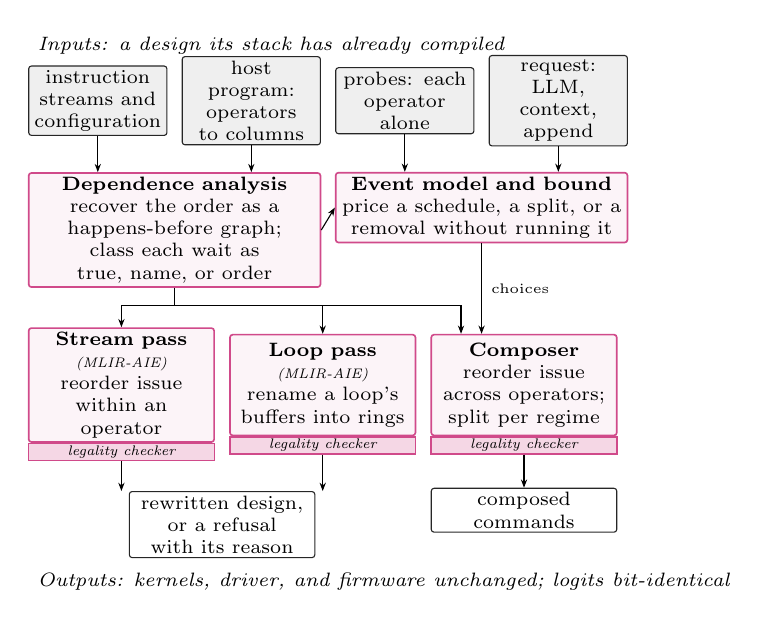
\begin{tikzpicture}[
    font=\scriptsize, >={Stealth[length=3pt]}, line width=0.4pt,
    inp/.style={draw=ink, fill=host!20, rounded corners=1pt, inner sep=1.5pt, align=center, text width=16.5mm, minimum height=7.2mm},
    comp/.style={draw=ours, line width=0.6pt, fill=ours!6, rounded corners=1pt, inner sep=1.5pt, align=center},
    rw/.style={comp, text width=22.5mm, minimum height=12.8mm},
    chk/.style={draw=ours, line width=0.6pt, fill=ours!22, inner sep=0.8pt, align=center, font=\tiny\itshape, minimum width=23.6mm},
    outp/.style={draw=ink, rounded corners=1pt, inner sep=1.5pt, align=center, text width=22.5mm, minimum height=5mm},
  ]
  % ---- inputs
  \node[inp] (i1) {instruction streams and configuration};
  \node[inp, right=1.8mm of i1] (i2) {host program: operators to columns};
  \node[inp, right=1.8mm of i2] (i3) {probes: each operator alone};
  \node[inp, right=1.8mm of i3] (i4) {request: LLM, context, append};
  \node[font=\scriptsize\itshape, anchor=south west] at ($(i1.north west)+(0,0.2mm)$) {Inputs: a design its stack has already compiled};
  % ---- analysis and model
  \node[comp, text width=36mm, anchor=north] (ana) at ($(i1.south)!0.5!(i2.south)+(0,-4.0mm)$)
    {\textbf{Dependence analysis}\\recover the order as a happens-before graph; class each wait as true, name, or order};
  \node[comp, text width=36mm, anchor=north] (mod) at ($(i3.south)!0.5!(i4.south)+(0,-4.0mm)$)
    {\textbf{Event model and bound}\\price a schedule, a split, or a removal without running it};
  \foreach \i/\t in {i1/ana, i2/ana, i3/mod, i4/mod} { \draw[->] (\i.south) -- (\i.south |- \t.north); }
  \draw[->] (ana.east) -- (mod.west);
  % ---- rewrites, each behind a legality checker
  \node[rw, anchor=north west] (spass) at ($(ana.south west)+(0,-5.0mm)$) {\textbf{Stream pass} {\tiny\itshape(MLIR-AIE)}\\reorder issue within an operator};
  \node[rw, right=1.8mm of spass] (lpass) {\textbf{Loop pass} {\tiny\itshape(MLIR-AIE)}\\rename a loop's buffers into rings};
  \node[rw, right=1.8mm of lpass] (cmp) {\textbf{Composer}\\reorder issue across operators; split per regime};
  \foreach \n in {spass, lpass, cmp} { \node[chk, anchor=north] (\n chk) at (\n.south) {legality checker}; }
  \coordinate (bus) at ($(ana.south)+(0,-2.2mm)$);
  \draw (ana.south) -- (bus);
  \draw[->] (bus) -| (spass.north);
  \draw[->] (bus) -| (lpass.north);
  \draw[->] (bus) -| ($(cmp.north)+(-8mm,0)$);
  \draw[->] (mod.south) -- node[right, font=\tiny] {choices} (mod.south |- cmp.north);
  % ---- outputs
  \node[outp, anchor=north] (o1) at ($(spasschk.south)!0.5!(lpasschk.south)+(0,-4.2mm)$) {rewritten design, or a refusal with its reason};
  \node[outp, anchor=north] (o2) at ($(cmpchk.south)+(0,-4.2mm)$) {composed commands};
  \draw[->] (spasschk.south) -- (spasschk.south |- o1.north);
  \draw[->] (lpasschk.south) -- (lpasschk.south |- o1.north);
  \draw[->] (cmpchk.south) -- (o2.north);
  \node[font=\scriptsize\itshape, anchor=north west] at ($(spass.south west |- o1.south)+(0,-0.6mm)$)
    {Outputs: kernels, driver, and firmware unchanged; logits bit-identical};
\end{tikzpicture}
\end{document}
